% This is auto-generated file: do not edit!
% Exported from microMathematics Plus, version 2.19.0


Now we plot several functions given in
the polar coordinate system. Each
point in this system is determined by
a distance r from the origin and the
angle f from the x-axis.
\begin{center}\begin{tabular}{c} 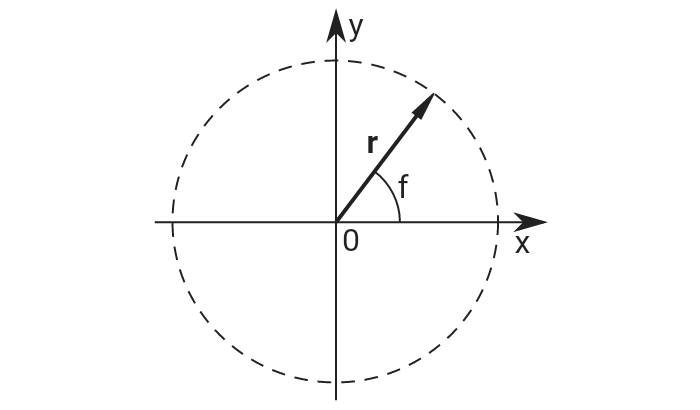
\includegraphics[resolution=320]{graphics/polar_plot_fig1.png} \end{tabular}\end{center}

The angle f is our independent variable
that is changed as follows:
\begin{center}\begin{tabular}{c}
  $f := \left[ 0.01,\, 0.05 \,..\, 300 \right]$
\end{tabular}\end{center}

The distance r(f) is our dependent
variable. Having a pair of f and r, we
can transform it to the Cartesian
coordinates x and y using sine and
cosine functions:
\begin{center}\begin{tabular}{cc}
  $x(r) := r \cdot cos \left( f\right) $ &
  $y(r) := r \cdot sin \left( f\right) $ \cr
\end{tabular}\end{center}

\subsection{A snail}

We will define our polar function in
three steps. The first expression
defines a ''wheel'':
\begin{center}\begin{tabular}{ccc}
  $A := 1.1$ &
  $B := 1.271$ &
  $q := 2$ \cr
\end{tabular}\end{center}
\begin{center}\begin{tabular}{c}
  $r1(f) := A + 2 \cdot {sin \left( B \cdot f\right) }^{q}$
\end{tabular}\end{center}

To plot this function, we add the plot
box using the ''New element'' button
in the action bar or ''Add function
plot'' button from the tool bar:
\begin{center}\begin{tabular}{c} 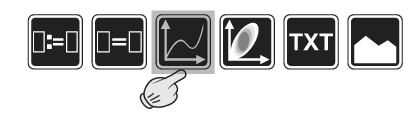
\includegraphics[resolution=320]{graphics/polar_plot_fig2.png} \end{tabular}\end{center}

Instead of f and r, we use here
previously defined rules for x and y
transformation, where r1(f) is used as
a symbolic argument for these rules:
\begin{center}\begin{tabular}{c} 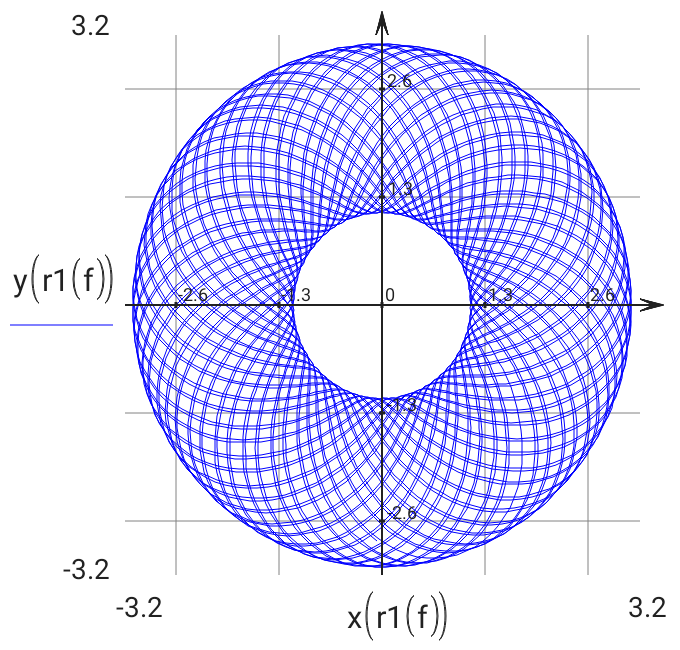
\includegraphics[resolution=320]{graphics/polar_plot_fig3.png} \end{tabular}\end{center}

Next, we can modify this wheel as
follows:
\begin{center}\begin{tabular}{c}
  $r2(f) := A + 2 \cdot {sin \left( B \cdot f + 1 \cdot r1 \left( f\right) \right) }^{q}$
\end{tabular}\end{center}
\begin{center}\begin{tabular}{c} 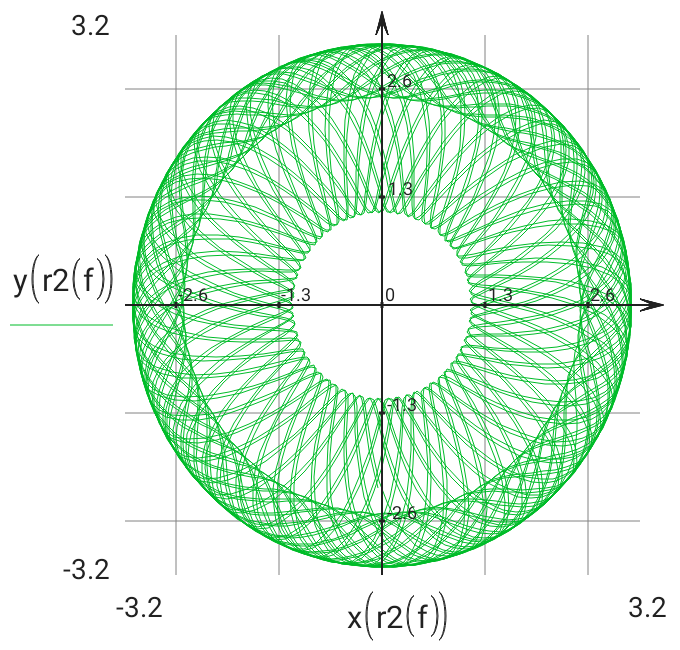
\includegraphics[resolution=320]{graphics/polar_plot_fig4.png} \end{tabular}\end{center}

Finally, we scale the last function
r2(f) using a float to integer
conversion that looks like a step
function. As a result, we obtain a
nice snail:
\begin{center}\begin{tabular}{c}
  $r(f) := r2 \left( f\right)  \cdot floor \left( f\right)  / 10$
\end{tabular}\end{center}
\begin{center}\begin{tabular}{c} 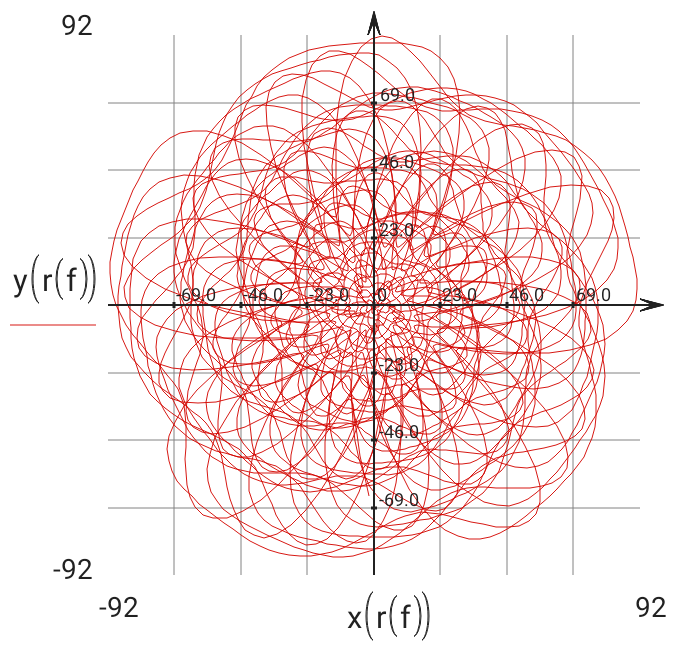
\includegraphics[resolution=320]{graphics/polar_plot_fig5.png} \end{tabular}\end{center}

\subsection{Japanese Maple}

Japanese Maple is well known for its
attractive leaf shapes and colors.
Such a leaf can be described
mathematically and plotted as a curve
in the polar coordinate system:
\begin{center}\begin{tabular}{c}
  $f := \left[ 0.01,\, 0.02 \,..\, 100 \right]$
\end{tabular}\end{center}
\begin{center}\begin{tabular}{cc}
  $x(r) := r \cdot cos \left( f\right) $ &
  $y(r) := r \cdot sin \left( f\right) $ \cr
\end{tabular}\end{center}
\begin{center}\begin{tabular}{c}
  $s1(f) := \left( 1 + sin \left( f\right)  \right) \cdot \left( 1 - 0.9 \cdot  \left| sin \left( 4 \cdot f\right)  \right|  \right)$
\end{tabular}\end{center}
\begin{center}\begin{tabular}{c}
  $s2(f) := 0.9 + 0.05 \cdot cos \left( 200 \cdot f\right) $
\end{tabular}\end{center}
\begin{center}\begin{tabular}{c}
  $r(f) := floor \left( f\right)  \cdot s1 \left( f\right)  \cdot s2 \left( f\right)  + random \left( 2\right)  - 1$
\end{tabular}\end{center}
\begin{center}\begin{tabular}{c} 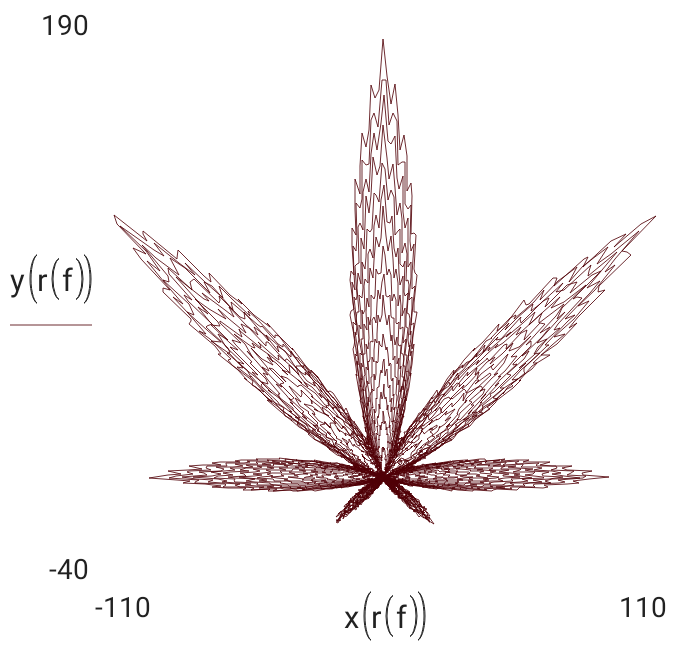
\includegraphics[resolution=320]{graphics/polar_plot_fig6.png} \end{tabular}\end{center}

http://en.wikipedia.org/wiki/Acer\_palmatum